\documentclass[10pt,a4paper,twocolumn]{article}
\usepackage[margin=16mm,columnsep=6mm,footskip=7mm]{geometry}
\usepackage[T1]{fontenc}
\usepackage{lmodern,microtype,amsmath,amssymb,booktabs,array,tabularx}
\usepackage{tikz}
\usetikzlibrary{arrows.meta,positioning}
\usepackage{caption,titlesec,url}
\usepackage[hidelinks]{hyperref}
\hypersetup{pdftitle={Divide-and-Conquer at Million-Scale: Closest-Pair Search and Integer Multiplication},pdfauthor={Fadil Faisal, M.Arham Usman, Khizer Sheikh},pdfsubject={CS2009 Design and Analysis of Algorithms, Submission 3}}
\captionsetup{font=small,labelfont=bf,skip=4pt}
\titleformat{\section}{\large\bfseries}{\thesection}{0.5em}{}
\titleformat{\subsection}{\normalsize\bfseries}{\thesubsection}{0.5em}{}
\titlespacing*{\section}{0pt}{9pt}{4pt}
\titlespacing*{\subsection}{0pt}{6pt}{3pt}
\setlength{\parindent}{0pt}
\setlength{\parskip}{4pt}
\setlength{\textfloatsep}{8pt}
\setlength{\intextsep}{7pt}
\setlength{\tabcolsep}{3pt}
\hyphenation{Karatsuba Tauri}
\raggedbottom
\renewcommand{\arraystretch}{1.13}
\newcolumntype{Y}{>{\raggedright\arraybackslash}X}
\newcommand{\file}[1]{\texttt{#1}}
% Generated by scripts/make_report_data.py
\newcommand{\CPMillionRadix}{53.6375}
\newcommand{\IMMillion}{33.0359}

\begin{document}
\twocolumn[{
\centering
{\LARGE\bfseries Divide-and-Conquer at Million-Scale\par}
\vspace{3pt}
{\large Closest-Pair Search and Integer Multiplication\par}
\vspace{7pt}
{Fadil Faisal (24K-0635) \quad M.Arham Usman (24K-1016)\par}
{Khizer Sheikh (24K-0520)\par}
\vspace{3pt}
{\small CS2009 -- Design and Analysis of Algorithms \;|\; BCS-5F\par}
{\small Instructor: Anaum Hamid \;|\; Submission 3 \;|\; November 20, 2026\par}
\vspace{10pt}
}]

\section*{Abstract}
We developed a desktop system for two-dimensional closest-pair search and nonnegative integer multiplication, combining custom divide-and-conquer algorithms with reproducible inputs and an explanatory interface. The system processes ten geometric and ten arithmetic datasets, including one million points and one million digits per operand. A standalone release-mode runner reuses the application kernels to measure computation separately from file handling and visualization. All 20 datasets pass independent result checks. On the million-size uniform cases, median times are \CPMillionRadix\,ms for closest-pair search with radix preprocessing and \IMMillion\,ms for multiplication. The experiments also expose the different costs of duplicate points, unbalanced operands and zero multiplication.

\section{Introduction}
Large inputs make exhaustive comparison and elementary arithmetic costly. Closest-pair search by testing every pair needs quadratic work; balanced schoolbook multiplication also has a quadratic digit-operation count. Divide and conquer reduces these costs by reusing structure between subproblems. Our project brings both algorithms into one workflow: deterministic input generation, file selection, batch execution and inspectable results. The evaluation covers the prescribed 20 datasets, including degenerate geometry and arithmetic edge cases, rather than only uniform random inputs.

\section{System Design}
Figure~\ref{fig:system} summarizes the implemented application. The React interface invokes Rust through Tauri. File processing runs in background tasks; batches progress in file order and retain individual errors. Rayon parallelizes sufficiently large recursive subproblems. The interface shows closest-pair coordinates and distance, or a product preview with a full-product copy action. Inputs of at most 101 points or 101 digits per operand receive bounded, paginated explanations.

\begin{figure}[ht]
\centering
% Editable vector figure; compiled directly by LaTeX/TikZ.
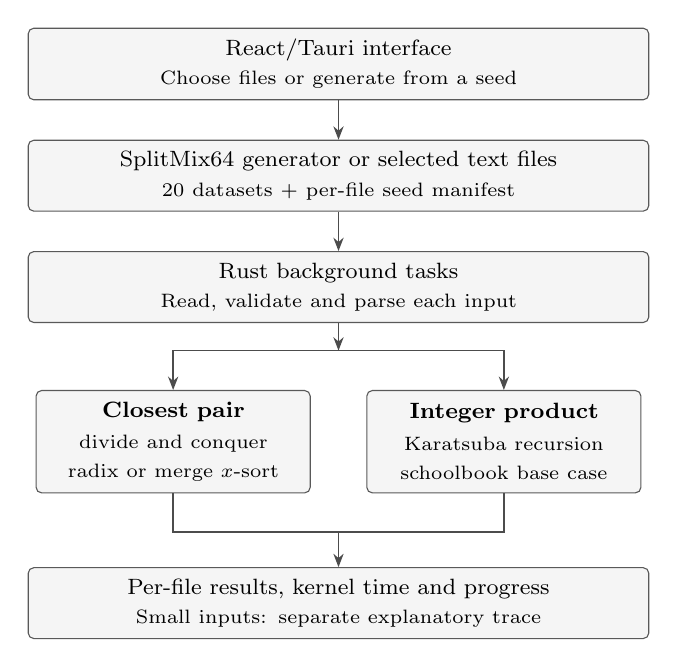
\begin{tikzpicture}[
  font=\footnotesize,
  box/.style={draw=black!65, rounded corners=2pt, fill=black!4,
    align=center, inner sep=4pt, text width=76mm, minimum height=9mm},
  alg/.style={draw=black!65, rounded corners=2pt, fill=black!4,
    align=center, inner sep=4pt, text width=32mm, minimum height=13mm},
  flow/.style={-{Stealth[length=1.7mm,width=1.3mm]}, semithick, draw=black!70}
]
\node[box] (ui) {React/Tauri interface\\[1pt]
  {\scriptsize Choose files or generate from a seed}};
\node[box,below=5mm of ui] (gen) {SplitMix64 generator or selected text files\\[1pt]
  {\scriptsize 20 datasets + per-file seed manifest}};
\node[box,below=5mm of gen] (parse) {Rust background tasks\\[1pt]
  {\scriptsize Read, validate and parse each input}};
\node[alg,below=8.5mm of parse,xshift=-21mm] (cp) {\textbf{Closest pair}\\[2pt]
  {\scriptsize divide and conquer}\\[1pt]{\scriptsize radix or merge $x$-sort}};
\node[alg,below=8.5mm of parse,xshift=21mm] (im) {\textbf{Integer product}\\[2pt]
  {\scriptsize Karatsuba recursion}\\[1pt]{\scriptsize schoolbook base case}};
\node[box,below=31mm of parse] (out) {Per-file results, kernel time and progress\\[1pt]
  {\scriptsize Small inputs: separate explanatory trace}};
\coordinate (split) at ([yshift=-3.5mm]parse.south);
\draw[flow] (ui.south) -- (gen.north);
\draw[flow] (gen.south) -- (parse.north);
\draw[flow] (parse.south) -- (split);
\draw[flow] (split) -| (cp.north);
\draw[flow] (split) -| (im.north);
\coordinate (collect) at ([yshift=4.5mm]out.north);
\draw[semithick,draw=black!70] (cp.south) -- (cp.south |- collect)
  -- (im.south |- collect) -- (im.south);
\draw[flow] (collect) -- (out.north);
\end{tikzpicture}

\caption{Application data flow. The standalone experiment runner calls copies of the same Rust kernels.}
\label{fig:system}
\end{figure}

\textbf{Closest pair.} A custom radix or merge sort orders points by $x$. Recursion divides this order by position, solves both halves and merges them by $y$. A middle strip is scanned using squared-distance bounds; the geometric packing argument keeps the combine work linear~\cite{wayne2005}. With a 16-point leaf solved by a direct y-ordered scan,
\[
T(n)=2T(n/2)+O(n)=O(n\log n).
\]
The radix option uses up to six passes over transformed 64-bit floating-point keys, skipping constant-digit passes and already-sorted inputs. Its linear preprocessing does not change the full algorithm's asymptotic bound. Merge sorting and recursive search use parallel branches from 16,384 points.

\textbf{Integer multiplication.} Decimal operands become little-endian base-$10^9$ limbs. Karatsuba replaces four half-size products with three~\cite{karatsuba1962}, giving
\[
T(m)=3T(m/2)+O(m)=O(m^{\log_2 3}),
\]
for balanced $m$-limb inputs. The implementation uses schoolbook multiplication when the shorter operand has at most 64 limbs, chunks strongly unbalanced operands, and parallelizes balanced recursion from 4,096 padded limbs. Zero returns immediately after conversion. Small-input explanations are separate teaching runs with lower cutoffs; they are not traces of the timed optimized execution.


\section{Experimental Setup}
\textbf{Environment and protocol.} Measurements use an AMD Ryzen 5 5600 (6 cores, 12 logical processors), approximately 16\,GiB RAM, Windows 11, Rust 1.99.1 and 12 Rayon workers. The standalone Rust runner contains locally copied generator and algorithm modules; interface-specific type metadata is removed, while the computational logic is retained. Release compilation uses optimization level 3, LTO and one codegen unit. Each configuration receives one warm-up and five measured runs; tables report their medians.

Closest-pair timing includes working allocation, the selected $x$-sort, recursion and the final square root. Multiplication timing includes arithmetic and its working allocation, but excludes decimal-to-limb conversion and product formatting. Both exclude file reading, parsing, independent verification, interface work and the separate explanation run. These are kernel measurements, not user-visible end-to-end latency. The application reports whole microseconds; the standalone runner additionally retains the same durations in nanoseconds, although the underlying clock does not resolve individual nanoseconds.

\textbf{Reproducible generation.} Each file uses \mbox{SplitMix64}~\cite{vigna2015} with its own state. With base seed $b=20261110$, \file{cp}$i$ uses $b+i-1$ and \file{im}$i$ uses $b+9+i$, for $i=1,\ldots,10$. Unsigned arithmetic wraps at 64 bits. Real draws use the upper 53 random bits divided by $2^{53}$; bounded integer draws use rejection sampling before reduction. Real coordinates are serialized to six decimal places. Grid and power-of-ten cases are deterministic, although their seeds are still recorded. All ten previously submitted small files match the regenerated copies byte for byte. Tables~\ref{tab:cpdata} and~\ref{tab:imdata} list each file's size, range and construction.

\begin{table}[ht]
\caption{Closest-pair inputs. $U$ denotes independent uniform draws; listed ranges describe generation, not observed extrema.}
\label{tab:cpdata}
\small
\begin{tabularx}{\columnwidth}{@{}lrY@{}}
\toprule
File & Points & Construction / coordinate range\\
\midrule
cp01 & $10^3$ & $x,y\sim U[0,10^6)$\\
cp02 & $10^4$ & Same uniform construction\\
cp03 & $10^5$ & Same uniform construction\\
cp04 & $10^6$ & Same uniform construction\\
cp05 & $10^6$ & Ten centers uniform in $[0,10^6)^2$; choose one uniformly per point, add offsets $U[-1000,1000)$ per axis, clip to $[0,10^6]$\\
cp06 & $10^6$ & Integer $x,y\in\{0,\ldots,255\}$; duplicates guaranteed\\
cp07 & $10^5$ & $x=500000$; $y\sim U[0,10^6)$\\
cp08 & $10^5$ & $250\times400$ grid; spacing 10; $x\in[0,2490]$, $y\in[0,3990]$\\
cp09 & $10^6$ & $1000\times1000$ grid; spacing 1000; injected middle pair (below)\\
cp10 & 101 & Uniform as cp01; explanation case\\
\bottomrule
\end{tabularx}
\end{table}

For cp09, the background grid spans $[0,999000]^2$. Two points are replaced by $(499499.999500,500000)$ and $(499500.000500,500000)$, placing a distance-$0.001$ pair across the median division. Uniform coordinates may round to the endpoint $10^6$ when written to six decimals. Each closest-pair text file starts with its point count, followed by one coordinate pair per line.

\begin{table}[ht]
\caption{Multiplication inputs. $R_d$ is a random $d$-digit integer with no leading zero.}
\label{tab:imdata}
\small
\begin{tabularx}{\columnwidth}{@{}lrrY@{}}
\toprule
File & Left digits & Right digits & Construction\\
\midrule
im01 & $10^3$ & $10^3$ & Two $R_{1000}$\\
im02 & $10^4$ & $10^4$ & Two $R_{10000}$\\
im03 & $10^5$ & $10^5$ & Two $R_{100000}$\\
im04 & $10^6$ & $10^6$ & Two $R_{1000000}$\\
im05 & $10^6$ & 10 & Left $R_{1000000}$; right $R_{10}$\\
im06 & $10^5$ & $10^5$ & Left $10^{100000}-1$ (all nines); right $R_{100000}$\\
im07 & 99,999 & 99,999 & Sparse: $77.5\%$ zero digits in both\\
im08 & $10^6$ & $10^6$ & Both $10^{999999}$\\
im09 & 1 & $10^6$ & Left operand $0$; right operand $R_{1000000}$\\
im10 & 101 & 101 & Two $R_{101}$; explanation case\\
\bottomrule
\end{tabularx}
\end{table}

For $R_d$, the leading digit is uniform on $1$--$9$ and each remaining digit is uniform on $0$--$9$, so $10^{d-1}\le R_d<10^d$. The two operands consume successive draws from the file's RNG. For im07, a nonleading digit is forced to zero with probability $3/4$; otherwise it is drawn uniformly from $0$--$9$. Its total zero probability is therefore $0.775$, with a nonzero leading digit. Multiplication files contain exactly two decimal lines.

\textbf{Independent correctness checks.} A separate sweep-line implementation verifies closest-pair minima using integer microcoordinates and exact squared distances; brute force checks small synthetic cases. A reported pair must occur in the input and achieve the reference minimum, allowing floating-point rounding and alternative tied pairs. Python arbitrary-precision multiplication checks each complete product exactly. These verification-only library operations never participate in the measured algorithms. Construction-specific checks include cp06 distance 0, cp08 distance 10, cp09 distance $0.001$, im08 product $10^{1999998}$ and im09 product 0. Verification compared full coordinates and complete products before summarizing the results.


\section{Results and Discussion}
% Generated from retained raw measurements; do not edit by hand.
All 20 input datasets passed independent verification, and all 27 copied Rust module tests passed. Both sorting configurations returned the same closest distances. Tables~\ref{tab:cpresults} and~\ref{tab:imresults} cover every prescribed file; verification used the returned coordinates and full decimal products.
\begin{table}[ht]
\caption{Closest-pair results: median kernel time in milliseconds (five runs). Distances are rounded for display.}
\label{tab:cpresults}
\small\centering
\begin{tabular}{@{}lrrr@{}}
\toprule
File & Merge (ms) & Radix (ms) & Distance\\
\midrule
cp01 & 0.1109 & 0.0702 & 315.635262\\
cp02 & 1.8678 & 1.2577 & 93.0324356\\
cp03 & 5.7468 & 5.0096 & 7.46221113\\
cp04 & 56.6059 & 53.6375 & 1.18885955\\
cp05 & 48.1578 & 44.7065 & 0.00373680775\\
cp06 & 37.1170 & 31.3648 & 0\\
cp07 & 5.5224 & 5.5892 & 0.000373999996\\
cp08 & 3.0149 & 2.9098 & 10\\
cp09 & 31.3902 & 35.3318 & 0.00100000005\\
cp10 & 0.0050 & 0.0097 & 7135.47551\\
\bottomrule
\end{tabular}
\end{table}
\begin{table}[ht]
\caption{Multiplication results: median kernel time and independently verified product length.}
\label{tab:imresults}
\small\centering
\begin{tabular}{@{}lrr@{}}
\toprule
File & Time (ms) & Product digits\\
\midrule
im01 & 0.0037 & 2,000\\
im02 & 0.1573 & 20,000\\
im03 & 1.2367 & 200,000\\
im04 & 33.0359 & 2,000,000\\
im05 & 0.4002 & 1,000,009\\
im06 & 1.3598 & 200,000\\
im07 & 1.2957 & 199,997\\
im08 & 32.1531 & 1,999,999\\
im09 & $\approx 0$ & 1\\
im10 & 0.0002 & 202\\
\bottomrule
\end{tabular}
\end{table}

\textbf{Example solutions.} cp04 returns $(984624.842563,\allowbreak 656374.534981)$ and $(984626.014180,\allowbreak 656374.736725)$. The full im10 product is shown below; line breaks separate consecutive digits:
\begin{quote}\scriptsize\ttfamily\raggedright
387289230164751802962022188871589393807826277241\\253168102200088490460117015739642406363146955021\\606529983911458448887140801670488726086089186701\\926934089760598603100748919454153734062149613836\\9629803660
\end{quote}

\textbf{Sorting and geometry.} Radix preprocessing has the lower median in 7 of ten cases. For cp04 it reduces median time by 5.2\% relative to merge preprocessing, but merge is faster on cp07, cp09 and cp10. Thus the observed advantage depends on input order, distribution and fixed costs. The clustered and duplicate cases are faster than the million-point uniform case in this run; finding a duplicate does not eliminate the remaining recursive merges.
The construction checks agree with the outputs: cp06 returns zero, cp08 returns 10, and cp09 returns approximately 0.001. Its computed value, 0.0010000000475, reflects binary floating-point subtraction. The exact-coordinate reference confirms the intended pair. Tied grid or duplicate inputs need not produce a unique pair.

\textbf{Operand shape and scaling.} From $10^5$ to $10^6$ random digits, multiplication time grows by $26.7\times$, versus about $10^{1.585}\approx38.5$ for a purely asymptotic sequential model. Parallel thresholds and fixed costs prevent interpreting this as a direct exponent estimate. im05 is much faster because its ten-digit operand occupies two limbs and selects the schoolbook path. im08 still performs balanced recursion despite its sparse operands; it is not handled by a dedicated power-of-ten shortcut.
For im09 the five retained samples are 0, 0, 0, 100 and 100 ns. The median is below the observed timer resolution, not evidence of zero execution cost. Reading and converting its million-digit operand still takes work outside the kernel timer. im10 likewise uses a schoolbook leaf in the timed run, even though its separate explanation illustrates Karatsuba recursion.

\textbf{Measurement limits.} cp04 radix samples span 51.82--54.28\,ms; im04 samples span 32.97--33.42\,ms. Runs use a shared desktop, fixed case order, and no CPU-affinity or power-plan control. Five repeats support descriptive comparisons, not statistical significance or hardware-independent speedups. We did not measure peak memory or interface latency. Exact product checks cover full outputs, whereas closest-pair arithmetic remains subject to floating-point rounding.


\section{Conclusion}
The system completes the prescribed geometric and arithmetic workloads up to one million points and one million digits per operand, with independent checks of every dataset. The experiments connect divide-and-conquer complexity to implementation choices: preprocessing affects closest-pair time, while operand shape determines whether multiplication uses balanced Karatsuba, schoolbook arithmetic or the zero shortcut. Reproducible generation and independent checks support the reported results. The interface adds file selection, progress and small-input explanations without charging visualization work to the measured kernels.

\begingroup
\small
\setlength{\parskip}{0pt}
\bibliographystyle{unsrt}
\bibliography{references}
\endgroup
\end{document}
